% ****** Start of file apssamp.tex ******
%
%   This file is part of the APS files in the REVTeX 4.1 distribution.
%   Version 4.1r of REVTeX, August 2010
%
%   Copyright (c) 2009, 2010 The American Physical Society.
%
%   See the REVTeX 4 README file for restrictions and more information.
%
% TeX'ing this file requires that you have AMS-LaTeX 2.0 installed
% as well as the rest of the prerequisites for REVTeX 4.1
%
% See the REVTeX 4 README file
% It also requires running BibTeX. The commands are as follows:
%
%  1)  latex apssamp.tex
%  2)  bibtex apssamp
%  3)  latex apssamp.tex
%  4)  latex apssamp.tex
%
\documentclass[%
 reprint,
%superscriptaddress,
%groupedaddress,
%unsortedaddress,
%runinaddress,
%frontmatterverbose, 
%preprint,
%showpacs,preprintnumbers,
%nofootinbib,
%nobibnotes,
%bibnotes,
 amsmath,amssymb,
 aps,
%pra,
%prb,
%rmp,
%prstab,
%prstper,
%floatfix,
]{revtex4-1}

\usepackage{graphicx}% Include figure files
\usepackage{hepunits}% Include figure files
\usepackage{color}
\usepackage{dcolumn}% Align table columns on decimal point
\usepackage{bm}% bold math
%\usepackage{hyperref}% add hypertext capabilities
%\usepackage[mathlines]{lineno}% Enable numbering of text and display math
%\linenumbers\relax % Commence numbering lines

%\usepackage[showframe,%Uncomment any one of the following lines to test 
%%scale=0.7, marginratio={1:1, 2:3}, ignoreall,% default settings
%%text={7in,10in},centering,
%%margin=1.5in,
%%total={6.5in,8.75in}, top=1.2in, left=0.9in, includefoot,
%%height=10in,a5paper,hmargin={3cm,0.8in},
%]{geometry}

\begin{document}

\preprint{LCCPEB---}

\title{The International Linear Collider \\ A Global Project}% Force line breaks with \\
\thanks{Version 1.3}%

\author{Jim Brau}
% \altaffiliation[Also at ]{Physics Department, XYZ University.}%Lines break automatically or can be forced with \\
\author{etal}%
 \email{Second.Author@institution.edu}
\affiliation{%
 Authors' institution and/or address\\
% This line break forced with \textbackslash\textbackslash
}%

\collaboration{Linear Collider Collaboration}%\noaffiliation

\date{\today}% It is always \today, today,
             %  but any date may be explicitly specified

\begin{abstract}
Input from the International Linear Collider community for the European Strategy Update: supplementary material

\end{abstract}

\pacs{Valid PACS appear here}% PACS, the Physics and Astronomy
                             % Classification Scheme.
%\keywords{Suggested keywords}%Use showkeys class option if keyword
                              %display desired
\maketitle

%\tableofcontents

\section{\label{sec:intro}Introduction}
   5 pages Brau + Peskin
\section{\label{sec:ilc}ILC Machine Design}

  15 pages B. List + Michizono
  
  % CHAPTER ON ILC MACHINE
  
\section{\label{sec:runscenarios}ILC Running Scenarios}
   5 pages J. List
   % CHAPTER ON ILC RUNNING SCENARIOS

Amoung the advantages of $e^+e^-$ colliders is the ability to collect datasets with different center-of-mass energies and beam polarisation settings, according to the neeeds of the various physics measurements.
While each measurement has its prefered data-taking mode, the combination with datasets collected other beam energies and/or beam polarisations provide important robustness against systematic uncertainties.

Any physics projection will depend on the exact assumptions on the assumed running scenario, i.e.\ the integrated luminosity collected at each considered center-of-mass energy with each polarisation setting.


The interplay of different datasets has been studied in detail in~\cite{Barklow:2015tja}, with a special focus on optimising the Higgs precision measurements. 

{\color{red} HERE: Tables with integrated luminsoities and polarisation mit from~\cite{Barklow:2015tja}}

{\color{red} Time dependence: explain why need longer when starting at 250\,\GeV}

{\color{red} explain new beam parameters, cite machine staging report}


%%%%%%%%%%%%%%%%%%%%%%%%%%%%%%%%%%%%%%%%%%%%%%%%%%%%%%%%%%%%%%%%%%%%%%%%%
\begin{figure}
\begin{center}
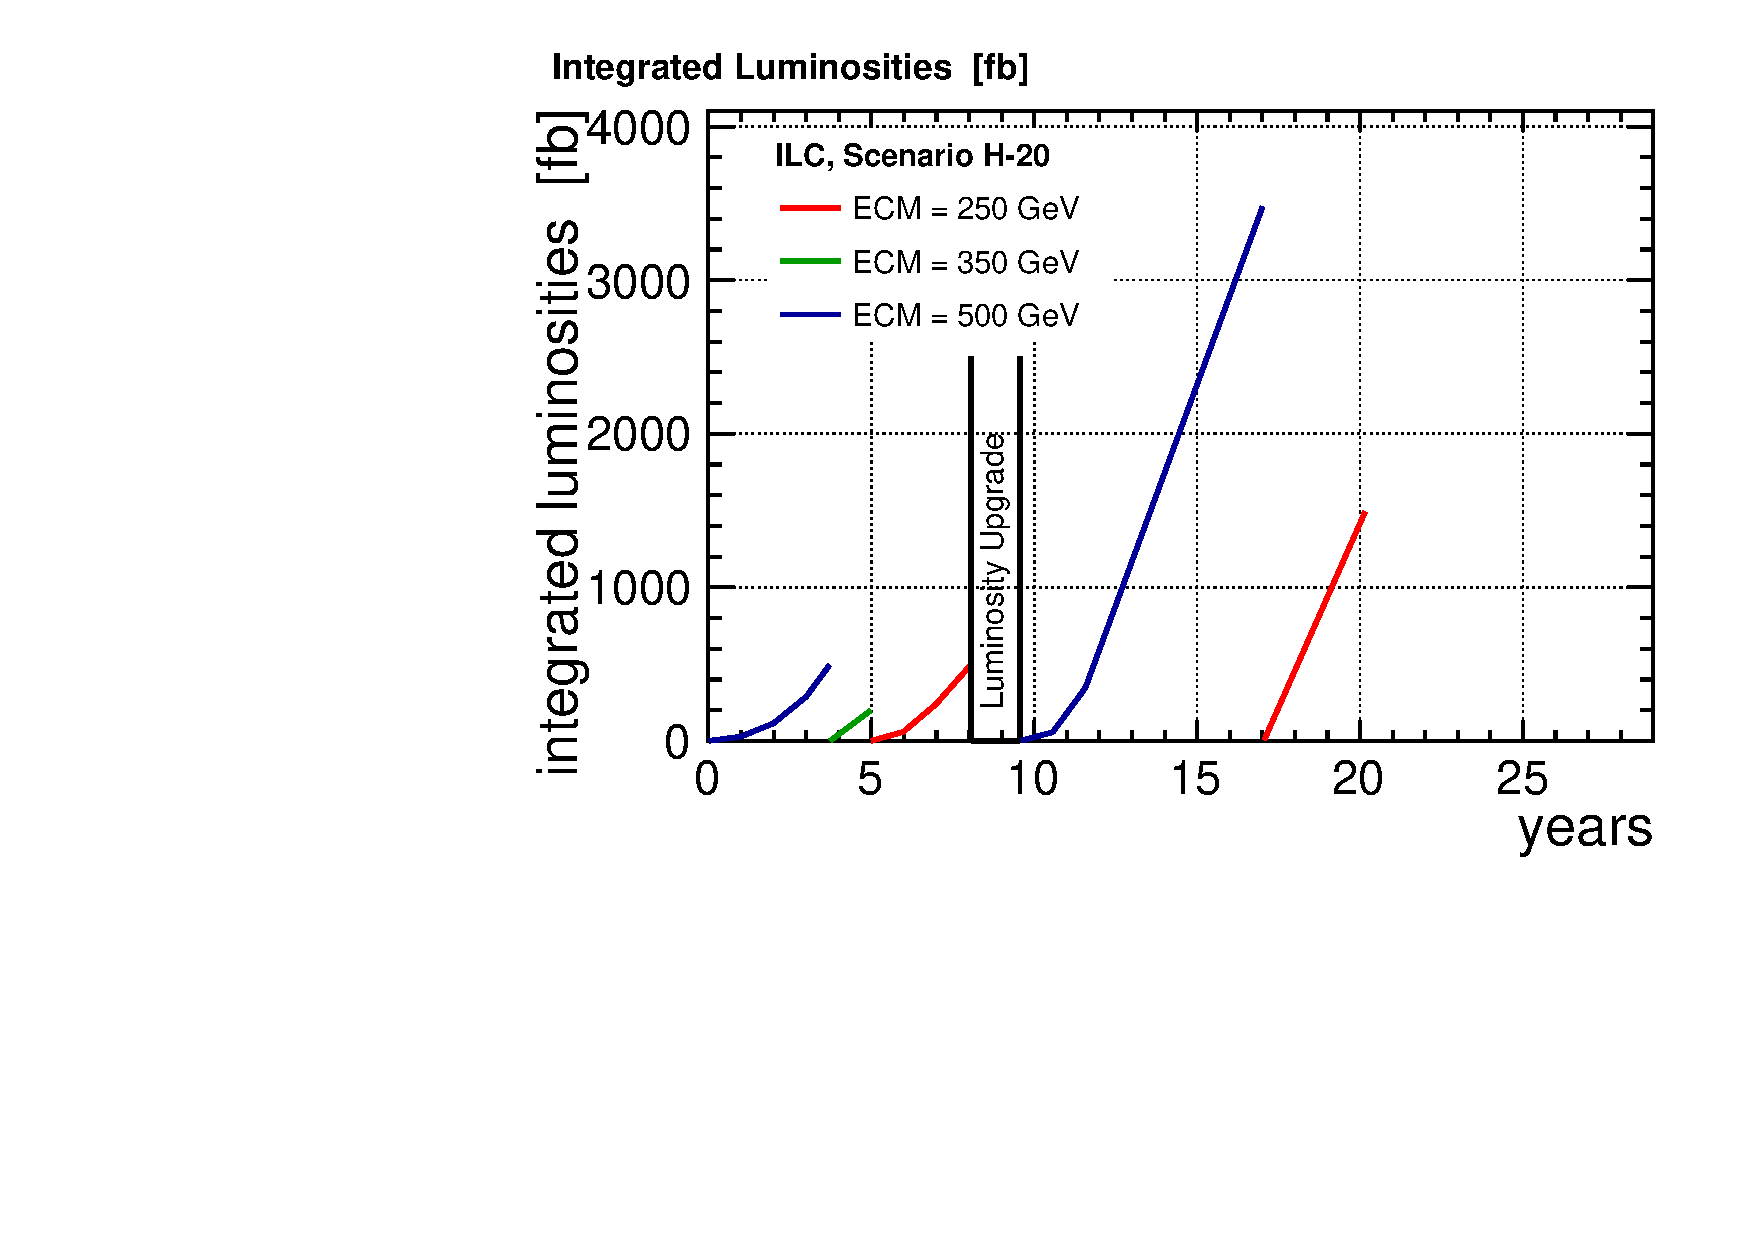
\includegraphics[width=0.75\hsize]{figs/lumi_H-20.pdf}
\end{center}
\caption{The nominal 20-year running program for the 500-GeV-ILC~\cite{Barklow:2015tja}.}
\label{fig:H20}
\end{figure}
%%%%%%%%%%%%%%%%%%%%%%%%%%%%%%%%%%%%%%%%%%%%%%%%%%%%%%%%%%%%%%%%%%%%%%%%%%%

%%%%%%%%%%%%%%%%%%%%%%%%%%%%%%%%%%%%%%%%%%%%%%%%%%%%%%%%%%%%%%%%%%%%%%%%%
\begin{figure}
\begin{center}
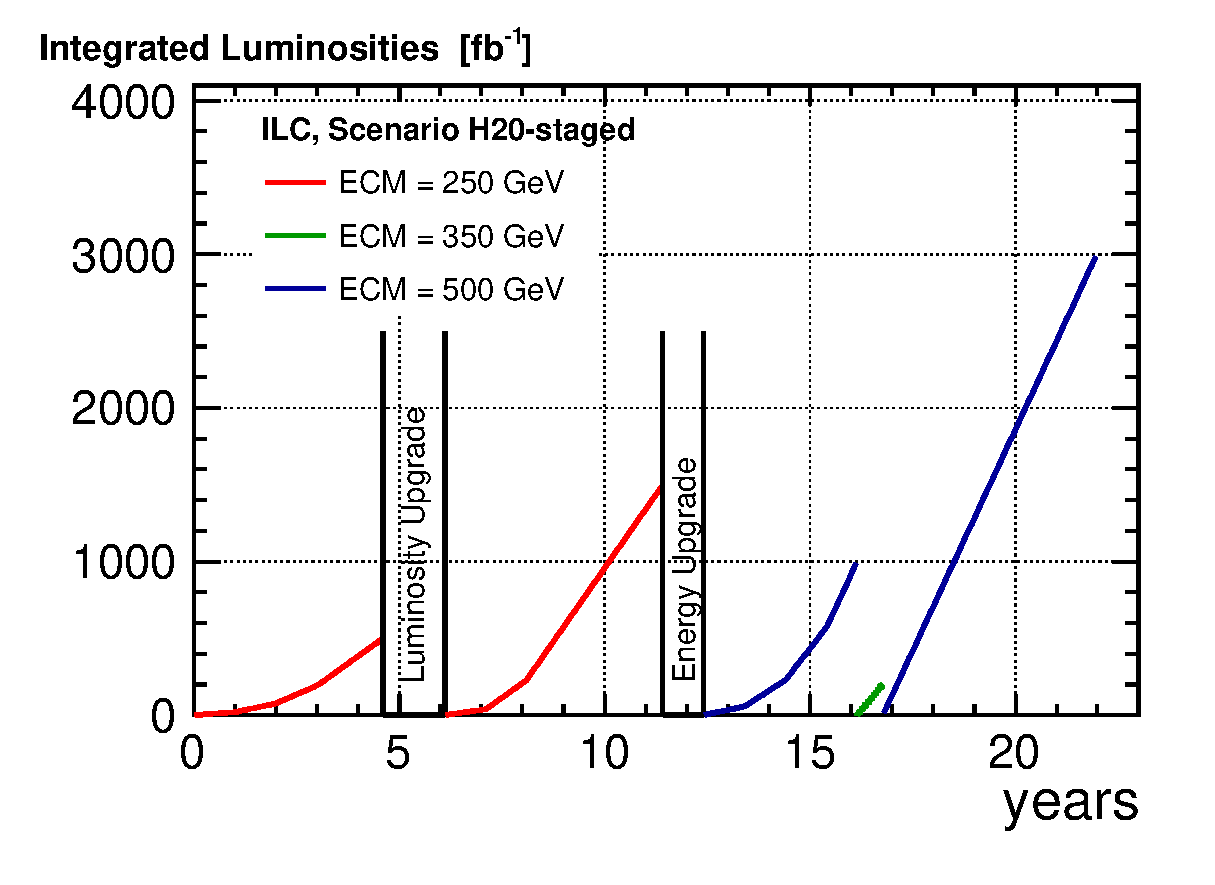
\includegraphics[width=0.75\hsize]{figs/lumi_H20-staged}
\end{center}
\caption{The nominal 22-year running program for the staged ILC, starting operation at 250\,\GeV ~\cite{ILC250}. The integrated luminosities are the same of for the original H20 scenario.}
\label{fig:H20}
\end{figure}
%%%%%%%%%%%%%%%%%%%%%%%%%%%%%%%%%%%%%%%%%%%%%%%%%%%%%%%%%%%%%%%%%%%%%%%%%%%

    
\section{\label{sec:physics}Physics Case (250 GeV) }
  10 pages Peskin
\section{\label{sec:detectors}Detectors }
  10 pages Behnke + White
\section{\label{sec:software}Software}
   10 pages Gaede + Miyamoto
\section{\label{sec:higgs}Physics Simulations: Higgs }
  20 pages Tian + J. List
\section{\label{sec:searches}Physics Simulations: Searches }
  5 pages Berggren
\section{\label{sec:ILC-HE}Program of the ILC beyond 250 GeV }
  10 pages Peskin, Fujii and Vos \\
  
  A key advantage of linear colliders is the possibility to upgrade the center-of-mass energy.
After finalizing the program discussed in Sections~\ref{sec:physics}, \ref{sec:higgs} and \ref{sec:searches} the linear collider can be expanded to explore energies well beyond 250~\gev{}. In this section, the potential of higher-energy operation is reviewed.

{\bf Upgradability:} While the energy reach of circular electron-positron colliders of a given circumference is limited by synchrotron radiation, a linear collider is very well suited to an upgrade of the center-of-mass energy after the 250~\gev{} program. This provides great flexibility to adapt or extend the program in response to new discoveries. The most obvious energy upgrade path is an extension of the linear accelerator (LINAC) sections of the colliders, which provides an increase in center-of-mass energy that is proportional to the length of the LINACs. The design of the ILC presented in the Technical Design Report~\cite{} thus reaches a center-of-mass energy of 500~\gev{} in a facility with a total length of 31~km. An even larger increase in center-of-mass energy may be achieved by exploiting advances in accelerator technology. The development of cavities with higher accelerating gradient can drive a significant increase in the energy while maintaining a compact infrastructure. The ILC TDR documents a possible extention to 1 TeV based on current superconducting RF technology~\cite{}. On a longer time scale, the advent of novel acceleration schemes such as plasma wakefield acceleration may open up the energy regime beyond several \tev. Thus, the linear collider facility can continue to contribute to particle physics over many decades. 



{\bf Measurement of the top-quark mass}

{\bf Top-quark electro-weak couplings}

{\bf Vector-boson fusion production of the Higgs boson}

{\bf Measurement of the Higgs self-coupling}


C. Adolphsen
et al.
, “The International Linear Collider Technical Design Report
-  Volume  3.I:  Accelerator  &  in  the  Technical  Design  Phase,”  arXiv:1306.6353
[physics.acc-ph].


\section{\label{sec:conclusion}Conclusion}





\end{document}
%
% ****** End of file apssamp.tex ******
